% !TEX program = lualatex
\documentclass[tikz, crop, border = {2pt 2pt 2pt 2pt}]{standalone}

\usetikzlibrary{calc, angles, quotes, patterns, decorations.pathreplacing, decorations.pathmorphing, calligraphy, arrows.meta}

\usepackage{pgfplots}

\begin{document}
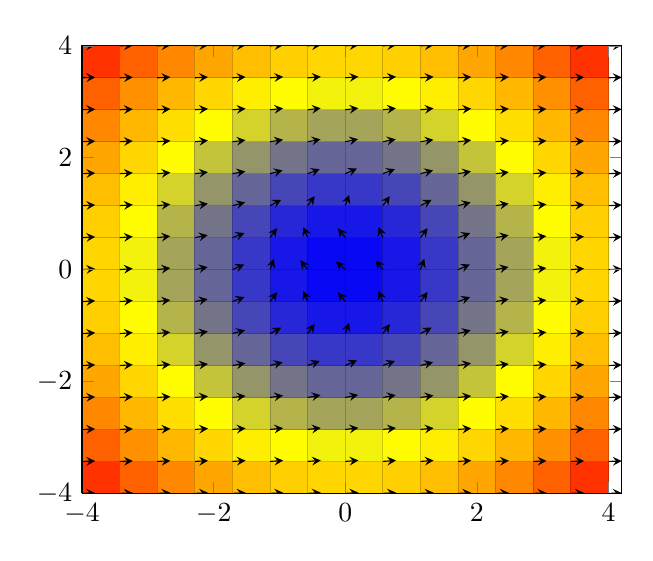
\begin{tikzpicture}
  \begin{axis}[
      domain = -4:4,
      view = {0}{90},
      clip = true,
      declare function = {
          func(\x, \y) = \x^2 + \y^2 - 1;
          norm(\x, \y) = sqrt(func(\x, \y)^2 + 1);
        }
    ]
    \addplot3[
      surf,
      samples = 15,
    ] {x^2 + y^2 - 1};
    \addplot3[
      samples = 15,
      quiver = {
          u = {func(x, y)/norm(x, y)},
          v = {1/norm(x, y)},
          scale arrows = 0.2
        },
      -stealth
    ] {0};
  \end{axis}
\end{tikzpicture}
\end{document}
